%%%%%%%%%%%%%%%%%%%%%%%%%%%%%%%%%%%%%%%%%%%%%%%%%%%%%%%%%%%%%%%%%%%%%%%%%%%%%%%

\chapter{PROPOSTA}\label{ch:prop}

Esta seção apresenta os objetivos do trabalho, bem como a problemática dos dados disponíveis atualmente e apresenta a estrutura que é proposta para solucionar o problema.

\section{Objetivos}\label{ch:prop:obj}

O objetivo principal deste trabalho é estabelecer um método para processamento de cubos de dados para a área espacial, para que o processamento de consultas OLAP sejam executadas de forma eficiente considerando-se a alta dimensionalidade, elevado número de tuplas, alto \textit{skew} e alta cardinalidade dos dados.
Como objetivos secundários, este trabalho visa:

\begin{enumerate}
\item Identificar quais são as consultas relevantes para os operadores de satélite, e quais são as atividades de análise que podem ser expressas como consultas;
\item Criar uma representação dimensional do cubo de dados apropriada para as consultas identificadas, mapeando as medidas que são necessárias e quais os seus tipos;
\item Implementar a representação com as medidas em algoritmos da literatura e coletar os resultados da execução das consultas relevantes para os operadores;
\item Avaliar os resultados da implementação dos algoritmos e mostrar qual das abordagens é mais apropriada para o cenário da operação.
\end{enumerate}

\section{Algoritmos de construção do cubo}\label{ch:prop:cube}

Esta proposta se concentra apenas na proposição de um algoritmo de computação do cubo de dados.
Uma das necessidades de usar algoritmos diferentes de cubo de dados está no número de dimensões que um certo cubo consegue realizar pesquisas: consultas com mais que 15 dimensões não são comummente(ou praticamente) executadas em alguns algoritmos, como o trabalho de~\citeonline{silva:2015:abordagensParaCubo} demonstra.

Os dados de telemetria de interesse possuem muito mais do que o limite comum de consultas em até 60 dimensões: com mais de 130 telemetrias para os satélites da família da SCD, e milhares para satélites maiores como o CBERS e o Amazônia, a execução de consultas complexas seria normalmente inviável nos algoritmos de construção do cubo tradicionais.

A figura~\ref{fig:qualistructure} mostra uma visão geral da estrutura proposta.
Seguindo a revisão feita an seção~\ref{ch:corr:cube}, o uso do \textit{FragCubing} seria adotado dadas as características altamente dimensionais e com alto \textit{skew} dos dados.
Porém seria adicionado um classificador de relacionamentos entre as telemetrias, que forneceria dados de entrada para o algoritmo do \textit{FragCubing} modificado, que decidirá como o cubo de dados resultante será construído.

\begin{figure}[!htb]
	\caption{Estrutura proposta}\label{fig:qualistructure}
	\vspace{2mm}
	\begin{center}
		\resizebox{14cm}{!}{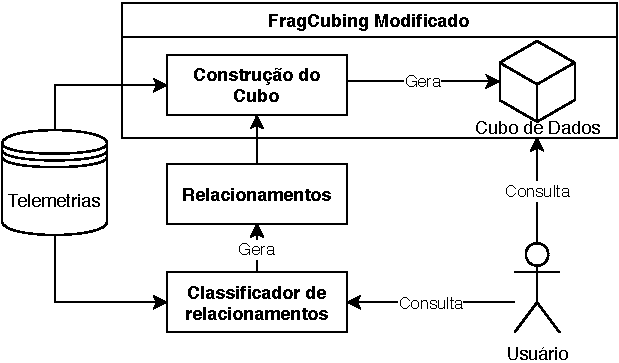
\includegraphics{Figuras/QualificationStructure.pdf}}
	\end{center}
	\vspace{1mm}
	\legenda{}
	\FONTE{Produção do autor.}
\end{figure}

\subsection{Funcionamento da estrutura}\label{ch:prop:cube:func}

Nesta estrutura, o fluxo de dados seria semelhante ao apresentado na seção~\ref{ch:corr:dataflow}, começando pela ingestão dos dados históricos, que seriam organizados e limpos conforme o necessário pelas características de cada satélite.
Este passo é necessário para garantir que dados são consistentes o bastante para que o algoritmo possa ser executado e obtenha resultados com maior qualidade.

O algoritmo de classificação seria então executado sobre os dados ingeridos, que teria os seus próprios resultados de classificação, também salvos.
Essas classificações e os dados ingeridos serviriam como entrada para o algoritmo do \textit{FragCubing} modificado, que utilizaria dos relacionamentos a sua discrição para montar um cubo de dados sobre os dados de telemetria.
É importante ressaltar que o \textit{FragCubing} é composto de um algoritmo de construção do cubo e um algoritmo de processamento das consultas, e esta proposta estaria alterando, em princípio, apenas o algoritmo de construção do cubo.

Neste passo, os relacionamentos seriam utilizados como necessário pelo algoritmo, pois a geração de todos os relacionamentos possíveis não é necessária em todo momento, e os relacionamentos mais relevantes seriam minerados pelo próprio algoritmo.
Disto o cubo de dados será construído, e o algoritmo pode então passar a responder consultas, seguindo o algoritmo do \textit{FragCubing}.

O usuário pode então consultar diretamente o classificador de relacionamentos para entender os relacionamentos entre as telemetrias, ou pode executar consultas sobre o cubo de dados gerado, dependendo da informação que lhe for necessária.
É importante ressaltar que as consultas diretas ao classificador são uma adição para a usabilidade da estrutura, não estando relacionadas diretamente com o algoritmo do \textit{FragCubing}.

